\chapter{三次曲面上的27条直线}

本章中，令 \(S \subset  {\mathbb{P}}^{3}\) 为一个由齐次三次多项式 \(f = f(X,Y,Z,T)\) 定义的非奇异三次曲面.我们考虑 \({\mathbb{P}}^{3}\) 中包含于 \(S\) 的直线 \(\ell\).

\section{非奇异性的推论}

\begin{proposition}
(a) 对 \(S\) 上的任意一点 \(P\)，至多有三条过 \(P\) 的直线包含于 \(S\)；若恰有两条或三条，则它们必共面.示意图如下：

\begin{center}
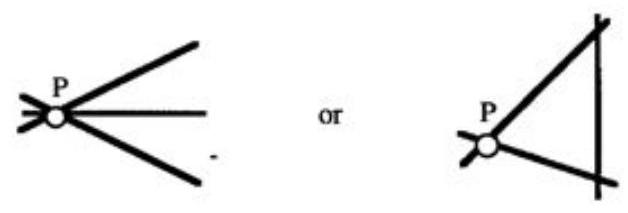
\includegraphics[max width=0.4\textwidth]{images/bo_d3lj80c601uc738kffi0_106_512_1114_628_213_0.jpg}
\end{center}
\hspace*{3em} 

图7.1:3条共点直线或三角形

(b) 每个平面 \(\Pi  \subset  {\mathbb{P}}^{3}\) 与 \(S\) 的交集是以下情形之一：

(i) 一个不可约三次曲线；或

(ii) 一条圆锥曲线和一条直线之并；或

(iii) 三条不同的直线之并.
\end{proposition}

\begin{proof}
(a) 若直线 \(\ell \subset S\) 且 \(P \in \ell\)，则 \(\ell = T_P\ell \subset T_PS\).因此，所有过 \(P\) 点且在 \(S\) 上的直线都包含在切平面 \(T_PS\) 内.由 (b) 可知，这样的直线至多有三条.

(b) 我们必须证明不可能出现重直线的情形.设平面 \(\Pi\) 的方程为 \(T=0\)，\(\Pi\) 中一直线 \(\ell\) 的方程为 \(Z=0\).若 \(\ell\) 是 \(S \cap \Pi\) 的一条重直线，则意味着 \(f\) 具有如下形式：
\[
f = Z^2 \cdot A(X,Y,Z,T) + T \cdot B(X,Y,Z,T),
\]
其中 \(A\) 为线性型，\(B\) 为二次型.此时，曲面 \(S: (f=0)\) 在满足 \(Z=T=B=0\) 的点处是奇异的.这是一个非空集合，因为它是二次型 \(B\) 在直线 \(\ell: (Z=T=0)\) 上的零点集.
\end{proof}

\begin{proposition}
曲面 \(S\) 上至少存在一条直线.
\end{proposition}

\begin{proof}
此命题有多种证明方法.一个经典论证是通过维数计算：\({\mathbb{P}}^{3}\) 中的直线构成一个4维簇，而一条直线 \(\ell\) 要被包含于 \(S\) 上，需要满足4个条件（因为 \(f\) 限制在 \(\ell\) 上是一个三次齐次多项式，其4个系数都必须为零）.要将此论证转化为严格证明，还需要一些工作，因为它先验地只表明直线集的维数 \(\ge 0\)，而非非空（详见 \cite[8.15]{MilesReid_UndergraduateAlgebraicGeometry} 对传统证明及其难点的讨论）.

我们也可以合理地假设该命题成立（即只关注那些包含直线的三次曲面）.现在，我们说明如何通过直接的坐标几何和消元法来证明命题 7.2.证明过程将占用接下来的三页，并分为四个步骤；如果你愿意，可以跳过（直接看命题 7.3）.

\textbf{步骤1（初步构造）} 对 \(S\) 上任意一点 \(P\)，\(S\) 与其切平面 \(T_PS\) 的交线是一个平面三次曲线 \(C = S \cap T_PS\).根据练习 6.7，该曲线在点 \(P\) 处奇异.我们假设 \(C\) 是不可约的，否则 \(P\) 就位于 \(S\) 的一条直线上，命题已然成立.此时，\(C\) 是一个有结点或尖点的三次曲线.我们可以选择适当的 \({\mathbb{P}}^{3}\) 坐标 \((X, Y, Z, T)\)，使得 \(T_PS\) 的方程为 \(T=0\)，\(P = (0,0,1,0)\)，且
\[
C: (XYZ = X^3 + Y^3) \text{ 或 } (X^2Z = Y^3).
\]
对给定的点 \(P \in S\)，交线 \(C\) 是有结点还是有尖点，取决于 \(f\) 在 \(P\) 点的二阶导数矩阵（即 Hessian 矩阵）.练习 7.3 对此有更详细的讨论，并证明了（在特征 \(\neq 2\) 时）尖点情形必在 \(S\) 的某点 \(P\) 处出现.为简便起见，我们在尖点情形下证明命题 7.2；原则上，结点情形的证明方法相同，但消元计算更为复杂（见练习 7.10）.因此，我们假设
\[
f = X^2Z - Y^3 + gT,
\]
其中 \(g = g_2(X,Y,Z,T)\) 是一个二次型.由于 \(S\) 在 \(P\) 点非奇异，我们可以假设 \(g(0,0,1,0) = 1\).

\textbf{步骤2（主要命题陈述）} 考虑 \(C \subset S\) 上的动点 \(P_\alpha = (1, \alpha, \alpha^3, 0)\).过 \(P_\alpha\) 的 \({\mathbb{P}}^{3}\) 中任意一条直线与补平面 \(\Pi: (X=0)\) 交于一点 \(Q = (0,Y,Z,T)\).我们用 \(\alpha\) 和 \(Q\) 的坐标来表示直线 \(P_\alpha Q\) 被包含于 \(S\) 的条件.将 \(f(\lambda P_\alpha + \mu Q)\) 按 \(\lambda\) 和 \(\mu\) 的幂次展开，得到
\[
P_\alpha Q \subset S \iff A(Y,Z,T) = B(Y,Z,T) = C(Y,Z,T) = 0,
\]
其中 \(A, B, C\) 是关于 \((Y, Z, T)\) 的 1, 2, 3 次齐次多项式，其系数与 \(\alpha\) 有关.

\textbf{主要命题}. 存在一个关于 \(\alpha\) 的 27 次首一“结式”多项式 \(R_{27}(\alpha)\)，使得
\[
R(\alpha) = 0 \iff A=B=C=0 \text{ 在 } {\mathbb{P}}^{2} \text{ 中有公共零点 } (\eta:\zeta:\tau).
\]
该命题证明了命题 7.2，因为它意味着对于 \(R\) 的每一个根 \(\alpha\)，都存在平面 \(\Pi\) 中的一点 \(Q = (0:\eta:\zeta:\tau)\)，使得直线 \(P_\alpha Q\) 包含于 \(S\).这里的思路是基于练习 1.10 的标准消元法计算；证明的其余部分将致力于明确写出 \(A, B, C\) 以证明此命题.

\textbf{步骤3（极化形式）} 定义 \(f\) 的极化形式 \(f_1\)，它是一个关于两组变量 \((X,Y,Z,T)\) 和 \((X',Y',Z',T')\) 的多项式，定义如下：
\[
f_1(X,Y,Z,T; X',Y',Z',T') = \frac{\partial f}{\partial X} X' + \frac{\partial f}{\partial Y} Y' + \frac{\partial f}{\partial Z} Z' + \frac{\partial f}{\partial T} T'.
\]
根据切空间的定义（见 (6.4) 和 (6.10)），对于 \(P=(X,Y,Z,T) \in S\) 和 \(P \neq Q=(X',Y',Z',T') \in {\mathbb{P}}^{3}\)，我们显然有
\[
f_1(P;Q) = 0 \iff \text{直线 } PQ \text{ 在点 } P \text{ 处与 } S \text{ 相切.}
\]
显然，
\[
f(\lambda P + \mu Q) = \lambda^3 f(P) + \lambda^2\mu f_1(P;Q) + \lambda\mu^2 f_1(Q;P) + \mu^3 f(Q),
\]
因此，对于 \(P \neq Q \in {\mathbb{P}}^{3}\)，以下四个条件
\[
f(P) = f_1(P;Q) = f_1(Q;P) = f(Q) = 0
\]
是直线 \(\ell = PQ\) 包含于曲面 \(S: (f=0)\) 的充要条件.从几何角度看，这些条件表明 \(\ell\) 在 \(P\) 和 \(Q\) 两点都与 \(S\) 相切，因此 \(f|_\ell\) 在这两点都有重根.由命题 1.8 可推得 \(\ell \subset S\).

对于 \(f = X^2Z - Y^3 + gT\)，其极化形式为
\[
f_1 = 2XZ \cdot X' - 3Y^2 \cdot Y' + X^2 \cdot Z' + g(X,Y,Z,T) \cdot T' + T g_1.
\]
这里 \(g_1 = g_1(X,Y,Z,T; X',Y',Z',T')\) 是以同样方式定义的 \(g\) 的极化形式.由于 \(g\) 是二次型，\(g_1\) 是对称双线性型，满足 \(g_1(P,P) = 2g(P)\).

代入 \(P_\alpha = (1, \alpha, \alpha^3, 0)\) 和 \(Q = (0,Y,Z,T)\)，我们得到直线 \(P_\alpha Q \subset S\) 的方程组为 \(A=B=C=0\)，其中
\begin{align*}
A &= Z - 3\alpha^2 Y + g(1, \alpha, \alpha^3, 0)T, \\
B &= -3\alpha Y^2 + g_1(1, \alpha, \alpha^3, 0; 0,Y,Z,T)T, \\
C &= -Y^3 + g(0,Y,Z,T)T.
\end{align*}

\textbf{步骤4（消元计算）} 现在我们从上述三个方程中消去 \(Y,Z,T\)，并关注 \(\alpha\) 的最高次幂.注意到由于 \(g(0,0,1,0)=1\)，我们有
\[
g(1, \alpha, \alpha^3, 0) = \alpha^6 + \dots = a^{(6)},
\]
其中 \(\dots\) 表示 \(\alpha\) 的低次项.因此，\(a^{(6)}\) 是一个 6 次首一多项式.方程 \(A=0\) 将 \(Z\) 表示为 \(Y\) 和 \(T\) 的线性组合：
\[
Z = 3\alpha^2 Y - a^{(6)}T.
\]
将此代入 \(B\)，并利用 \(g_1\) 的双线性性质，得到
\begin{align*}
B &= -3\alpha Y^2 + g_1(1, \alpha, \alpha^3, 0; 0, Y, 3\alpha^2 Y - a^{(6)}T, T)T \\
  &= b_0 Y^2 + b_1 YT + b_2 T^2,
\end{align*}
其中
\begin{align*}
b_0 &= -3\alpha, \\
b_1 &= g_1(1, \alpha, \alpha^3, 0; 0, 1, 3\alpha^2, 0) = 6\alpha^5 + \dots, \\
b_2 &= g_1(1, \alpha, \alpha^3, 0; 0, 0, -a^{(6)}, 1) = -2\alpha^9 + \dots.
\end{align*}
类似地，将 \(Z\) 的表达式代入 \(C\)，并展开二次型 \(g\)，得到
\begin{align*}
C &= -Y^3 + g(0, Y, 3\alpha^2 Y - a^{(6)}T, T)T \\
  &= c_0 Y^3 + c_1 Y^2T + c_2 YT^2 + c_3 T^3,
\end{align*}
其中
\begin{align*}
c_0 &= -1, \\
c_1 &= g(0, 1, 3\alpha^2, 0) = 9\alpha^4 + \dots, \\
c_2 &= g_1(0, 1, 3\alpha^2, 0; 0, 0, -a^{(6)}, 1) = -6\alpha^8 + \dots, \\
c_3 &= g(0, 0, -a^{(6)}, 1) = \alpha^{12} + \dots.
\end{align*}
现在，根据练习 1.10 的结式理论，\(B\) 和 \(C\) 有公共零点 \((\eta:\tau)\) 当且仅当它们的 Sylvester 行列式为零：
\[
\det \begin{vmatrix}
-3\alpha & 6\alpha^5 & -2\alpha^9 & & \\
& -3\alpha & 6\alpha^5 & -2\alpha^9 & \\
& & -3\alpha & 6\alpha^5 & -2\alpha^9 \\
-1 & 9\alpha^4 & -6\alpha^8 & \alpha^{12} & \\
& -1 & 9\alpha^4 & -6\alpha^8 & \alpha^{12}
\end{vmatrix} = 0.
\]
该行列式是关于 \(\alpha\) 的多项式，不难看出其首项来自于取行列式中每个元素的首项：
\[
\det \begin{vmatrix}
-3\alpha & 6\alpha^5 & -2\alpha^9 & & \\
& -3\alpha & 6\alpha^5 & -2\alpha^9 & \\
& & -3\alpha & 6\alpha^5 & -2\alpha^9 \\
-1 & 9\alpha^4 & -6\alpha^8 & \alpha^{12} & \\
& -1 & 9\alpha^4 & -6\alpha^8 & \alpha^{12}
\end{vmatrix} = \alpha^{27} \cdot \det \begin{vmatrix}
-3 & 6 & -2 & & \\
& -3 & 6 & -2 & \\
& & -3 & 6 & -2 \\
-1 & 9 & -6 & 1 & \\
& -1 & 9 & -6 & 1
\end{vmatrix}
\]
（行列式中的 `2` 应该是 `-2`）经过计算，这个 \(5 \times 5\) 的常数行列式的值为 1，所以
\[
\text{结式} = \alpha^{27} + \dots.
\]
这便完成了主要命题的证明.
\end{proof}

\begin{proposition}
给定一条直线 \(\ell \subset S\)，恰好存在 5 对直线 \((\ell_i, \ell_i')\)，它们是 \(S\) 中与 \(\ell\) 相交的直线，且满足：
\begin{enumerate}
    \item[(i)] 对 \(i=1, \dots, 5\)，\(\ell \cup \ell_i \cup \ell_i'\) 共面；
    \item[(ii)] 对 \(i \neq j\)，\((\ell_i \cup \ell_i') \cap (\ell_j \cup \ell_j') = \varnothing\).
\end{enumerate}
\end{proposition}

\begin{proof}
(摘自 \cite[p. 51]{Beauville_ComplexAlgebraicSurfaces}) 若 \(\Pi\) 是 \({\mathbb{P}}^{3}\) 中任一包含 \(\ell\) 的平面，则 \(\Pi \cap S = \ell \cup C\)，其中 \(C\) 是一条圆锥曲线（因为 \(f|_\Pi\) 可被 \(\ell\) 的方程整除）.该圆锥曲线可以是奇异的，也可以是非奇异的：

\begin{center}
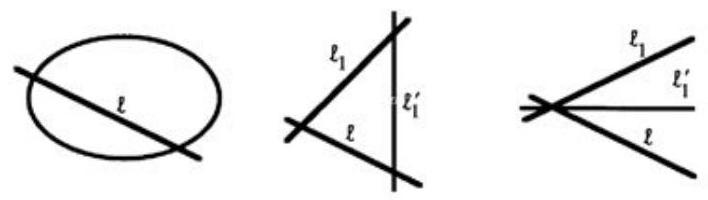
\includegraphics[max width=0.5\textwidth]{images/bo_d3lj80c601uc738kffi0_110_493_393_708_200_0.jpg}
\end{center}
\hspace*{3em} 

图7.2: 直线与圆锥曲线之并

我们必须证明，恰有 5 个不同的平面 \(\Pi_i \supset \ell\) 使得奇异情形（即圆锥曲线分解为两条直线）发生.性质 (ii) 中所述的不同平面内的直线互不相交，这是命题 7.1(a) 的直接推论.

假设 \(\ell\) 的方程为 \(Z=T=0\).那么我们可以将 \(f\) 展开为
\[
f = AX^2 + BXY + CY^2 + DX + EY + F, \quad (*)
\]
其中 \(A,B,C,D,E,F \in k[Z,T]\)，\(A,B,C\) 是线性型，\(D,E\) 是二次型，\(F\) 是三次型.如果我们将此方程视为变量在 \(X,Y\) 中的圆锥曲线，则其退化（即奇异）的条件是判别式为零：
\[
\Delta(Z,T) = \det \begin{pmatrix} 2A & B & D \\ B & 2C & E \\ D & E & 2F \end{pmatrix} = 4ACF + BDE - AE^2 - B^2F - CD^2 = 0.
\]
(这里我们假设特征 \(\neq 2\).在特征 2 的情况下，这是一个简单的练习.)

更准确地说，任何过 \(\ell\) 的平面都由 \(\Pi: (\mu Z = \lambda T)\) 给出.若 \(\mu \neq 0\)，我们可以设 \(\mu=1\)，即 \(Z = \lambda T\).然后用平面 \(\Pi\) 上的齐次坐标 \((X,Y,T)\) 表示，我们有 \(f|_\Pi = T \cdot Q(X,Y,T)\)，其中
\begin{multline*}
Q = A(\lambda,1)X^2 + B(\lambda,1)XY + C(\lambda,1)Y^2 \\
+ D(\lambda,1)TX + E(\lambda,1)TY + F(\lambda,1)T^2.
\end{multline*}
现在，\(\Delta(Z,T)\) 是一个关于 \(Z,T\) 的齐次五次多项式，因此根据代数基本定理（或命题 1.8），它有 5 个根（计重数）.为证明该命题，我们必须证明它没有重根.这同样是 \(S\) 非奇异性的一个推论.

\textbf{命题}. \(\Delta(Z,T)\) 只有单根.

\begin{proof}
假设 \(Z=0\) 是 \(\Delta\) 的一个根，并令 \(\Pi: (Z=0)\) 为对应的平面.我们必须证明 \(\Delta\) 不能被 \(Z^2\) 整除.根据上图，\(\Pi \cap S\) 是三条直线的并.根据这三条直线是否共点，我们可以调整坐标使得：
\begin{itemize}
    \item[(i)] \(\ell: (T=0), \ell_1: (X=0), \ell_1': (Y=0)\)（不共点，构成三角形）；
    \item[(ii)] \(\ell: (T=0), \ell_1: (X=0), \ell_1': (X=T)\)（共点）.
\end{itemize}
在情形 (i) 中，\(f = XYT + Zg\)，其中 \(g\) 是二次型.根据表达式 (*)，这意味着 \(B = T + aZ\)，且 \(Z\) 整除 \(A,C,D,E,F\).因此，在模 \(Z^2\) 的意义下，
\[
\Delta \equiv -B^2F \equiv -T^2F \pmod{Z^2}.
\]
此外，点 \(P=(0,0,0,1) \in S\)，\(S\) 在 \(P\) 点的非奇异性意味着 \(F\) 必须包含形如 \(cZT^2\) 且 \(c \neq 0\) 的项.特别地，\(Z^2\) 不整除 \(F\).因此，\((Z=0)\) 是 \(\Delta\) 的一个单根.

情形 (ii) 的计算是类似的（见习题 7.1）.
\end{proof}
\end{proof}

\begin{corollary}
1. \(S\) 上存在两条不相交的直线 \(\ell, m\).
2. \(S\) 是有理曲面（即与 \({\mathbb{P}}^{2}\) 双有理等价，见 (5.9)）.
\end{corollary}

\begin{proof}
(a) 根据命题 7.3(ii)，只需取 \(\ell_1\) 和 \(\ell_2\).

(b) 考虑 \(S\) 上两条不相交的直线 \(\ell, m\)，并定义如下的有理映射：
\[
\varphi: S \dashrightarrow \ell \times m \quad \text{和} \quad \psi: \ell \times m \dashrightarrow S.
\]
如果 \(P \in {\mathbb{P}}^{3} \setminus (\ell \cup m)\)，则存在唯一一条通过 \(P\) 且同时与 \(\ell\) 和 \(m\) 相交的直线 \(n\)，即
\[
P \in n, \quad \ell \cap n \neq \varnothing, \quad m \cap n \neq \varnothing.
\]
令 \(\Phi(P) = (\ell \cap n, m \cap n) \in \ell \times m\).这定义了一个态射
\[
\Phi: {\mathbb{P}}^{3} \setminus (\ell \cup m) \to \ell \times m,
\]
其在 \((Q,R) \in \ell \times m\) 上的纤维是 \({\mathbb{P}}^{3}\) 中的直线 \(QR\).定义 \(\varphi: S \dashrightarrow \ell \times m\) 为 \(\Phi\) 在 \(S\) 上的限制.

反之，对于 \((Q,R) \in \ell \times m\)，令 \(n\) 为 \({\mathbb{P}}^{3}\) 中的直线 \(n=QR\).根据命题 7.3，与 \(\ell\) 相交的 \(S\) 中的直线只有有限条.因此，对于几乎所有的 \((Q,R)\)，直线 \(n\) 与 \(S\) 交于三点 \(\{P,Q,R\}\)，其中 \(Q \in \ell\) 和 \(R \in m\) 是给定的点.因此，我们通过 \((Q,R) \mapsto P\) 定义了 \(\psi: \ell \times m \dashrightarrow S\).由于 \(P\) 的坐标是 \(Q,R\) 坐标的有理函数，故 \(\psi\) 是一个有理映射.

显然，\(\varphi\) 和 \(\psi\) 互为逆映射.
\end{proof}

\section{寻找所有S上的直线}

我们希望基于命题 7.3 给出的由一条直线 \(\ell\) 和 5 对不相交直线 \((\ell_i, \ell_i')\) 构成的图形，找出 \(S\) 上的所有直线.任何其他直线 \(n \subset S\) 必须与 \(i=1, \dots, 5\) 中的每一对 \((\ell_i, \ell_i')\) 之一恰好相交一次.这是因为在 \({\mathbb{P}}^{3}\) 中，\(n\) 与包含第 \(i\) 对直线的平面 \(\Pi_i\) 相交，而 \(\Pi_i \cap S = \ell \cup \ell_i \cup \ell_i'\).此外，\(n\) 不可能同时与 \(\ell_i\) 和 \(\ell_i'\) 相交，否则将与命题 7.1(a) 矛盾.解决剩余直线问题的关键是以下引理，它告诉我们 \(n\) 由其与 \(\ell_i\) 和 \(\ell_i'\) 中的哪一条相交唯一确定.这里，我们说一条直线 \(n\) 是直线 \(\ell\) 的一条“贯线”（transversal），如果 \(\ell \cap n \neq \varnothing\).

\begin{lemma}
如果 \({\ell}_{1},\ldots ,{\ell}_{4} \subset  {\mathbb{P}}^{3}\) 是四条互相不交的直线，则
\begin{itemize}
    \item 要么这四条直线 \(\ell_i\) 都位于一个光滑二次曲面上，\({\ell}_{1},\ldots ,{\ell}_{4} \subset  Q \subset  {\mathbb{P}}^{3}\).此时，它们有无穷多条公共贯线.
    \item 要么这四条直线 \(\ell_i\) 不位于任何二次曲面上.此时，它们有 1 条或 2 条公共贯线.
\end{itemize}
\end{lemma}

\begin{proof}
存在一个光滑二次曲面 \(Q \supset \ell_1, \ell_2, \ell_3\).对此有多种证明方法（见练习 7.2）.

\begin{center}
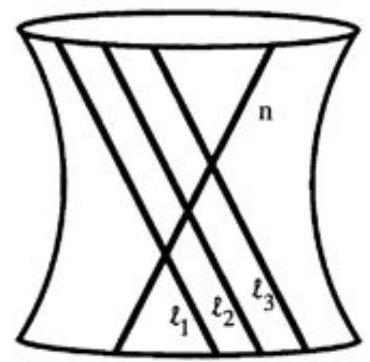
\includegraphics[max width=0.2\textwidth]{images/bo_d3lj80c601uc738kffi0_112_658_391_370_362_0.jpg}
\end{center}
\hspace*{3em} 

图7.3: 过三条不交直线的二次曲面

那么，在适当的坐标系中，\(Q\) 的方程为 \(XT-YZ=0\)，且 \(Q\) 上有两族直纹，或称母线.任何贯穿 \(\ell_1, \ell_2, \ell_3\) 的直线都必须位于 \(Q\) 中，因为它在 \(Q\) 上有三个点.现在，如果 \(\ell_4 \not\subset Q\)，则 \(\ell_4 \cap Q\) 为一个或两个点.通过这些点的另一族母线即为 \(\ell_1, \dots, \ell_4\) 的所有公共贯线.
\end{proof}

\section{27条直线}

设 \(\ell\) 和 \(m\) 是 \(S\) 中两条不相交的直线.如前所述，\(m\) 恰好与 5 对和 \(\ell\) 相交的直线中的每一对的一条相交.通过重新编号，我们假设 \(m\) 与 \(\ell_i\) 相交，其中 \(i=1, \dots, 5\).我们引入以下记号来表示与 \(\ell\) 或 \(m\) 相交的直线：

\begin{center}
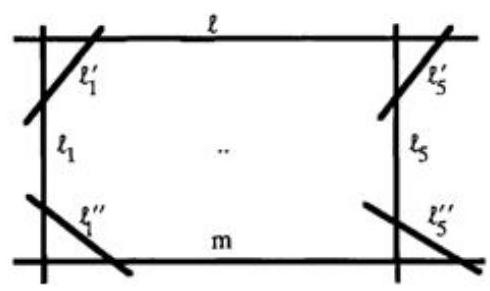
\includegraphics[max width=0.3\textwidth]{images/bo_d3lj80c601uc738kffi0_112_603_1306_490_291_0.jpg}
\end{center}
\hspace*{3em} 

图7.4: \(S_3 \subset {\mathbb{P}}^3\) 上的直线构型

因此，与 \(m\) 相交的 5 对直线是 \((\ell_i, \ell_i'')\)，其中 \(i=1, \dots, 5\).根据命题 7.3(ii) 对 \(m\) 的应用，对于 \(i \neq j\)，直线 \(\ell_i''\) 不与 \(\ell_j\) 相交.另一方面，\(S\) 中的每条直线必须与 \(\ell, \ell_j\) 或 \(\ell_j'\) 中的一条相交，因此 \(\ell_i''\) 必与 \(\ell_j'\) 相交，其中 \(i \neq j\).

\begin{proposition}
(I) 如果 \(n \subset S\) 是除这 17 条（\(\ell, m, \ell_i, \ell_i', \ell_i''\)）之外的任意直线，则 \(n\) 恰好与 \(\ell_1, \dots, \ell_5\) 中的三条相交.

(II) 反之，对于集合 \(\{1,2,3,4,5\}\) 中任意选择的 3 个元素 \(\{i,j,k\}\)，都存在唯一一条直线 \(\ell_{ijk} \subset S\) 与 \(\ell_i, \ell_j, \ell_k\) 相交.
\end{proposition}

\begin{proof}
(I) 给定 \(S\) 中的四条不相交直线，显然它们不可能都位于同一个二次曲面 \(Q\) 上，否则 \(Q \subset S\)，这与 \(S\) 的不可约性矛盾.

如果 \(n\) 与 \(\ge 4\) 条 \(\ell_i\) 相交，则根据引理 7.5，\(n\) 必为 \(\ell\) 或 \(m\)，这产生矛盾.如果 \(n\) 与 \(\le 2\) 条 \(\ell_i\) 相交，则它必与 \(\ge 3\) 条 \(\ell_i'\) 相交.因此，它与 \(\ell_2', \ell_3', \ell_4', \ell_5'\) 或 \(\ell_1, \ell_3', \ell_4', \ell_5'\) 之一相交.但如上所述，\(\ell\) 和 \(\ell_1''\) 是五条不相交直线 \(\ell_2', \ell_3', \ell_4', \ell_5', \ell_1\) 的两条公共贯线.因此，再次根据引理 7.5，如果 \(n\) 与其中 \(\ge 4\) 条相交，则 \(n\) 必为 \(\ell\) 或 \(\ell_1''\).这同样是矛盾.

(II) 根据命题 7.3，有 10 条直线与 \(\ell_1\) 相交.目前我们只考虑了其中的 4 条（即 \(\ell, \ell_1', m, \ell_1''\)）.其余 6 条直线必须恰好与剩下的 4 条直线 \(\ell_2, \dots, \ell_5\) 中的两条相交.而这样的选择恰好有 \(6 = \binom{4}{2}\) 种，因此它们必须全部出现.
\end{proof}

这给出了 \(S\) 上的所有直线为：
\[
\{\ell, m, \ell_i, \ell_i', \ell_i'', \ell_{ijk}\},
\]
其总数为
\[
1 + 1 + 5 + 5 + 5 + 10 = 27.
\]

\section{直线的构型}

另一种表述是，\(S\) 上的直线是 \(\ell, \ell_1, \dots, \ell_5, \ell_1', \dots, \ell_5'\)，以及另外 16 条与 \(\ell_1, \dots, \ell_5\) 相交奇数次的直线：
\begin{itemize}
    \item \(\ell_i''\) 只与 \(\ell_i\) 相交.
    \item \(\ell_{ijk}\) 只与 \(\ell_i, \ell_j, \ell_k\) 相交.
    \item \(m\) 与所有的 \(\ell_1, \dots, \ell_5\) 相交.
\end{itemize}
在我引入的记号中，很容易看出 \(S\) 的 27 条直线之间的相交关系如下：
\begin{itemize}
    \item \(\ell\) 与 \(\ell_1, \dots, \ell_5, \ell_1', \dots, \ell_5'\) 相交.
    \item \(\ell_1\) 与 \(\ell, m, \ell_1', \ell_1''\) 相交，并与 6 条 \(\ell_{1jk}\)（其中 \(\{j,k\} \subset \{2,3,4,5\}\)）相交.
    \item \(\ell_1'\) 与 \(\ell, \ell_1, \ell_j''\)（\(j \neq 1\)，4种选择）相交，并与 \(\ell_{ijk}\)（\(\{i,j,k\} \subset \{2,3,4,5\}\)，4种选择）相交.
    \item \(\ell_1''\) 与 \(m, \ell_1, \ell_j'\)（\(j \neq 1\)，4种选择）相交，并与 \(\ell_{ijk}\)（\(\{i,j,k\} \subset \{2,3,4,5\}\)，4种选择）相交.
    \item \(\ell_{123}\) 与 \(\ell_1, \ell_2, \ell_3, \ell_{145}, \ell_{245}, \ell_{345}, \ell_4', \ell_5', \ell_4'', \ell_5''\) 相交.
\end{itemize}
该组合构型有多种不同的表示形式，其中一些比此处给出的更具对称性；例如参见 \cite[pp. 122-128, 151-152]{SempleRoth_IntroductionToAlgebraicGeometry}.

\section{第7章习题}

\begin{exercise}
证明命题 7.3 中所声明的情形 (ii).[提示：如同情形 (i) 的证明，\(f = X(X-T)T + Zg\)，因此 \(A = T+aZ, D = -T^2 + Z\ell\)，其中 \(\ell\) 是线性的.于是 \(Z \mid B,C,E,F\)，且 \(Z \nmid D\).此外，\(S\) 在点 \((0,1,0,0)\) 处的非奇异性意味着 \(C=cZ\) 且 \(c \neq 0\).现在计算 \(\Delta(Z,T) \pmod{Z^2}\).]
\end{exercise}

\begin{exercise}
证明给定三条互相不交的直线 \(\ell_1, \ell_2, \ell_3 \subset {\mathbb{P}}^{3}\)，存在一个非奇异的二次曲面 \(Q \supset \ell_1, \ell_2, \ell_3\).[提示：在每条直线 \(\ell_i\) 上取三个点 \(P_i, P_i', P_i''\)，并如 (1.11) 或 (2.4) 所示，证明至少存在一个过这九个点的二次曲面 \(Q\).由此可知 \(\ell_i \subset Q\).现在证明 \(Q\) 不可能是奇异的：例如，如果 \(Q\) 是一对平面，会发生什么？]
\end{exercise}

\begin{exercise}[Hessian 矩阵]
设 \(f = f_d(x_0, \dots, x_n)\) 是关于 \(x_0, \dots, x_n\) 的 \(d\) 次齐次多项式，定义了超曲面 \(V: (f=0) \subset {\mathbb{P}}^{n}\).为简便起见，假设域的特征 \(\neq 2\) 且不整除 \(d-1\).记 \(f_{x_i} = \partial f/\partial x_i\) 和 \(f_{x_ix_j} = \partial^2 f/\partial x_i \partial x_j\) 分别为 \(f\) 的一阶和二阶偏导数.\(f\) 在点 \(P \in {\mathbb{P}}^{n}\) 处的泰勒展开为
\[
f = f(P) + f^{(1)}(x) + f^{(2)}(x) + \dots,
\]
其中 \(f^{(1)}\) 和 \(f^{(2)}\) 分别是线性和二次齐次多项式：
\[
f^{(1)} = \sum f_{x_i}(P) \cdot x_i \quad \text{和} \quad f^{(2)} = \frac{1}{2} \sum f_{x_ix_j}(P) \cdot x_i x_j.
\]
如果 \(P \in V\) 是一个奇异点，那么 \(f(P)\) 和 \(f^{(1)}\) 在 \(P\) 处为零，\(V\) 或 \(f\) 在 \(P\) 附近的性质由二次型 \(f^{(2)}\) 在二阶近似下决定.类似地，如果 \(P \in V\) 是一个非奇异点，那么 \(f\) 限制在超平面 \(T_PV\) 上的性质（或奇异超平面截面 \(V \cap T_PV\) 的性质）由 \(f^{(2)}\) 决定.定义 \(f\) 关于坐标 \(x_0, \dots, x_n\) 的 Hessian 矩阵为 \(H(f) = H(f,x) = \{f_{x_ix_j}\}_{i,j}\)，Hessian \(h(f) = h(f,x)\) 定义为其行列式 \(h(f) = \det H(f)\).

(i) 设 \(x_i' = \sum a_{ij}x_j\) 为一个射影坐标变换，\(A = (a_{ij})\) 是一个非奇异的 \((n+1) \times (n+1)\) 矩阵.若 \(g(x') = f(Ax)\)，证明 Hessian 矩阵的变换规律为
\[
H(g,x') = ({}^tA) H(f,x) A,
\]
其中 \({}^tA\) 为转置矩阵.由此推导出 \(h(g,x') = (\det A)^2 h(f,x)\).

(ii) 考虑如 (5.5) 中所述的仿射片 \(V_{(i)} \subset {\mathbb{A}}_{(i)}^{n}\)，设 \(P \in V_{(i)}\) 为非奇异点，\(\Pi = T_P V_{(i)}\) 为仿射切平面.记 \(\varphi\) 为定义方程 \(f/x_i^d\) 在 \(\Pi\) 上的限制.证明 \(\varphi\) 在 \(P\) 处的泰勒展开以一个非退化的二次型 \(\varphi^{(2)}\)（在 \(n-1\) 个变量中）开始，当且仅当 \(h(f)(P) \neq 0\).
[提示：利用 (i) 化简为 \(P=(1,0,\dots,0)\) 和 \(T_PV: (x_1=0)\).此时 \(\varphi^{(2)}\) 是射影 Hessian 矩阵 \(H(f)\) 的右下角 \((n-1) \times (n-1)\) 子矩阵.用 \(f_{x_i}(P)=0\)（\(i \neq 1\)）和欧拉公式 \(\sum_j f_{x_ix_j} x_j = (d-1)f_{x_i}\) 证明矩阵 \(H(f)\) 在第 0 行和第 0 列中恰有一个非零元.参见 \cite[p. 116]{Fulton_AlgebraicCurves}.]

(iii) 设 \(C: (f=0) \subset {\mathbb{P}}^{2}\) 为非奇异平面三次曲线.由 (ii) 推导出 \(P \in C\) 是一个拐点当且仅当 \(H(f)(P)=0\).Bézout 定理表明 \((f=H(f)=0) \subset {\mathbb{P}}^{2}\) 非空（参见 (1.9) 及 \cite[p. 112]{Fulton_AlgebraicCurves}）.

(iv) 设 \(S: (f=0) \subset {\mathbb{P}}^{3}\) 为非奇异三次曲面.对 \(P \in S\)，证明若 \(P\) 不在 \(S\) 的任何直线上，则交线 \(S \cap T_PS\) 为尖点三次曲线当且仅当 \(H(f)(P)=0\).由此推断存在尖点三次截面，正如命题 7.2 证明步骤 1 所需.
\end{exercise}

\begin{exercise}
(i) 证明若 \(P\) 是三次曲面 \(S\) 的一个奇异点，则至少存在一条直线 \(\ell \subset S\) 经过 \(P\)（且“一般情况下”有 6 条）.

(ii) 如果 \(X \subset {\mathbb{P}}^{4}\) 是一个非奇异的三次超曲面（三次三维簇）且 \(P \in X\)，那么至少存在一条直线 \(\ell \subset X\) 经过 \(P\)（通常有 6 条）.[提示：用 \(P=(1,0,\dots,0)\) 的坐标写出 \(X\) 的方程.]
\end{exercise}

\begin{exercise}
证明推论 7.4(b) 中的有理映射 \(\varphi: S \dashrightarrow \ell \times m\) 实际上是一个态射.证明它将 \(S\) 上的 5 条直线收缩为点.
\end{exercise}

\begin{exercise}
找出对角三次曲面（Fermat 三次曲面）
\[
S: (X^3 + Y^3 + Z^3 + T^3 = 0) \subset {\mathbb{P}}^{3}
\]
上的全部 27 条直线，可用形如 \((X = \rho Y)\) 的平面来寻找，其中 \(\rho^3=-1\).
\end{exercise}

\begin{exercise}
设 \(S \subset {\mathbb{P}}^{3}\) 是由 \(S: (f=0)\) 给出的三次曲面，其中
\[
f(X,Y,Z,T) = ZX^2 + TY^2 + (Z-d^2T)(Z-e^2T)(Z-f^2T),
\]
\(d,e,f\) 是 \(k\) 中不同的非零元素.\(\ell \subset S\) 是由 \(Z=T=0\) 给出的直线.通过类似命题 7.3 中考虑经过 \(\ell\) 的动平面，写出与 \(\ell\) 相交的 \(S\) 上的 10 条直线的方程.
\end{exercise}

\begin{exercise}[由 R. Casdagli 提出]
考虑在仿射坐标下由下式给出的三次曲面 \(S_{(0)} \subset {\mathbb{R}}^{3}\)：
\[
x^2 + y^2 + z^2 - 2xyz = 1 + \lambda^2, \quad (*)
\]
其中 \(\lambda \in \mathbb{R}, \lambda > 0\) 是常数.(i) 通过将 \((*)\) 重写为
\[
(x-yz)^2 = (y^2-1)(z^2-1) + \lambda^2,
\]
证明 \(S_{(0)}\) 有 4 个通向无穷远的管状区域.另一方面，相应的射影曲面 \(S \subset {\mathbb{P}}_{\mathbb{R}}^{3}\) 在无穷远处与三条直线 \(XYZ=0\) 相交.利用此信息描述 \(S\) 的拓扑结构.

(ii) 将 \((*)\) 视为以 \(z\) 为参数的 \((x,y)\) 平面上的动圆锥曲线方程，证明与平面 \((Z=0)\) 渐近相交的四对 \(S_{(0)}\) 上的直线由下式给出：
\begin{align*}
z = \mu, &\quad x = (\mu \pm \sqrt{\mu^2-1})y \\
z = -\mu, &\quad x = (-\mu \pm \sqrt{\mu^2-1})y;
\end{align*}
以及另外 8 条实直线，例如
\[
z=1, \quad x-y = \pm\lambda; \quad \text{和} \quad z=-1, \quad x+y = \pm\lambda,
\]
其中 \(\mu^2 = 1+\lambda^2\).
用计算机图形学或制作石膏模型来展示曲面 \(S_{(0)}\) 在 \({\mathbb{R}}^{3}\) 中的形态及其 24 条实直线.
\end{exercise}

\begin{exercise}[所有直线均为有理线的情形]
假设域 \(k\) 的特征 \(\neq 2\).设 \(S: (f=0)\) 是一个非奇异三次曲面，满足
\[
f = A(X,Y)T - B(X,Y)Z + (\text{含 } Z,T \text{ 的次数} \ge 2 \text{ 的项}).
\]
则 \(S\) 包含直线 \(\ell: (Z=T=0)\)，且在点 \(P=(1,\lambda,0,0)\) 处的切平面为 \(T_PS: A(1,\lambda)T = B(1,\lambda)Z\).

(i) 利用 \((X,Y)\) 和 \((Z,T)\) 的线性坐标变换，将 \(A,B\) 化简为 \(A=X^2+\Delta Y^2, B=XY\)（其中 \(\Delta \in k\)）；若 \(\Delta\) 是完全平方，则可化为 \(A=X^2, B=Y^2\).

(ii) 假设 \(S\) 也包含直线 \(m: (X=Y=0)\)，并且为简化符号，设 \(A=X^2, B=Y^2\).令 \(\ell_i\)（\(i=1,\dots,5\)）为 \(\ell\) 和 \(m\) 的 5 条公共贯线，记 \(P_i = (1, \lambda_i, 0, 0) = \ell_i \cap \ell\) 为 \(\ell\) 与 \(\ell_i\) 的交点.证明
\[
\ell_i: (Y = \lambda_i X, T = \lambda_i^2 Z) \quad \text{for } i=1,\dots,5,
\]
并且
\[
f = X^2T - Y^2Z + X(\sigma_5 Z^2 + \sigma_3 ZT + \sigma_1 T^2) - Y(\sigma_4 Z^2 + \sigma_2 ZT + T^2),
\]
其中 \(\sigma_1, \dots, \sigma_5\) 是 \(\lambda_1, \dots, \lambda_5\) 的初等对称多项式.

(iii) 求 \(S\) 上剩余的直线.[提示：\(\ell_i'\) 和 \(\ell_i''\) 包含在你已知的平面中.按照 (7.6) 中的论证，不难证明每条与 \(\ell_1, \ell_2, \ell_3\) 三条线相交的直线都可表示为 \((\tau_2 Z+T):X = (\tau_3 Z+\tau_1 T):Y = \alpha:\beta\)，其中 \(\tau_i\) 是 \(\lambda_1, \lambda_2, \lambda_3\) 的初等对称多项式.]
\end{exercise}

\begin{exercise}
本练习适合喜欢大量计算的读者，或有计算机代数系统辅助者.如果一个非奇异三次曲面 \(S\) 有一个结点三次曲线 \(C\) 作为截面，其方程可写为
\[
f = XYZ - X^3 - Y^3 + Tg.
\]
设 \(P_\alpha = (\alpha, \alpha^2, 1+\alpha^3, 0)\)（\(\alpha \neq 0, \infty\)）是 \(C\) 上的动点，及 \(Q=(0,Y,Z,T)\).然后按照命题 7.2 步骤 3，将 \(f(\lambda P_\alpha + \mu Q)\) 展开为 \(f\) 的极化形式，证明直线 \(P_\alpha Q \subset S\) 当且仅当 \(A=B=C=0\)，其中
\begin{align*}
A &= (-3\alpha^2+1)Y + \alpha^2 Z + g(\alpha, \alpha^2, 1+\alpha^3, 0)T; \\
B &= \alpha YZ - 3\alpha^2 Y^2 + g_1(\alpha, \alpha^2, 1+\alpha^3, 0; 0,Y,Z,T)T; \\
C &= -Y^3 + g(0,Y,Z,T)T.
\end{align*}
证明存在一个关于 \(\alpha\) 的 27 次“结式”多项式 \(R_{27}(\alpha)\)，使得对于 \(\alpha \neq 0\)，
\[
R(\alpha) = 0 \iff A=B=C=0 \text{ 在 } {\mathbb{P}}^{2} \text{ 中有公共零点 } (\eta:\zeta:\tau).
\]
[提示：从 \(A=0\) 解出 \(Z\)（这会在分母中引入 \(\alpha^2\)），将 \(Z\) 代入 \(B\) 和 \(C\)，得到关于 \(Y,T\) 的二次和三次二元多项式，然后用 Sylvester 行列式消去 \(Y,T\).此处的难点在于，当 \(\alpha \to 0\) 或 \(\alpha \to \infty\) 时，\(P_\alpha\) 趋于结点，此时 \(A,B,C\) 有平凡公共解，导致结式的首项和末项系数计算变得复杂.你需要仔细计算以确定其确切次数和系数.]
\end{exercise}
